\chapter{基于代码审查图的代码结构可视化和质量评估}
\section{引言}


在软件开发过程中,开发者通常会经历多个阶段。在项目的初始阶段,开发者需要阅读和理解已有的代码,这是熟悉软件项目的第一步。然而,对于大型项目而言,由于项目代码量庞大,涉及的模块和功能众多,这一过程通常需要耗费大量的时间和精力。除此之外,开发者在对软件进行修改时,如添加新功能或修复缺陷,通常需要深入了解修改代码的上下文信息。如果对上下文理解不清晰,可能会导致变更不完全或不准确,进而影响软件质量。在软件开发的后期,开发者往往需要作为代码审查者参与到代码审查过程中。代码审查的主要目的是评估变更后的代码是否符合质量标准,是否能够顺利地合并到主分支中。这一过程不仅在协作开发中至关重要,也是确保软件质量的有效手段。然而,代码审查往往需要投入大量的时间和精力\cite{花子涵2024代码审查自动化研究综述}。审查者不仅需要对变更的代码本身进行分析,还需要理解这些代码所处的上下文,才能做出正确的评估。

因此,无论是作为开发者还是审查者,理解软件项目的结构和代码是至关重要的。只有深入掌握软件的整体架构和各模块之间的关系,才能在后续的开发和审查过程中保证代码质量。然而,传统的代码阅读和理解方式不仅需要消耗大量的时间和精力,还难以确保高效性和准确性,尤其是在面对庞大复杂的代码库时。

为了提高代码理解的效率并减少人为错误,本文提出了一种基于代码审查图的代码架构和质量信息可视化的方法。通过将项目中的各个方法和全局变量表示为图的节点,用边表示方法与方法之间、方法与全局变量之间的依赖关系、耦合关系和变更影响关系,从而形成一个结构化的代码关系图。这样的图形化展示方式能够帮助开发者和审查者从宏观的角度掌握整个软件项目的架构和各个模块之间的关系,进而提升对代码的理解效率。通过这种方式,开发者和审查者可以更直观地识别出项目中的关键部分及其相互依赖关系,从而在变更和审查过程中更高效地评估代码的质量和影响。

\section{基于代码度量的代码质量度量模型}

\subsection{代码质量度量模型}

代码质量度量模型用于评估和量化软件代码质量,本文研究对象是方法以及模块的代码质量,我们选取以下4个方面的质量属性和14个对应的度量元来进行衡量。

\begin{figure}[h]
\centering
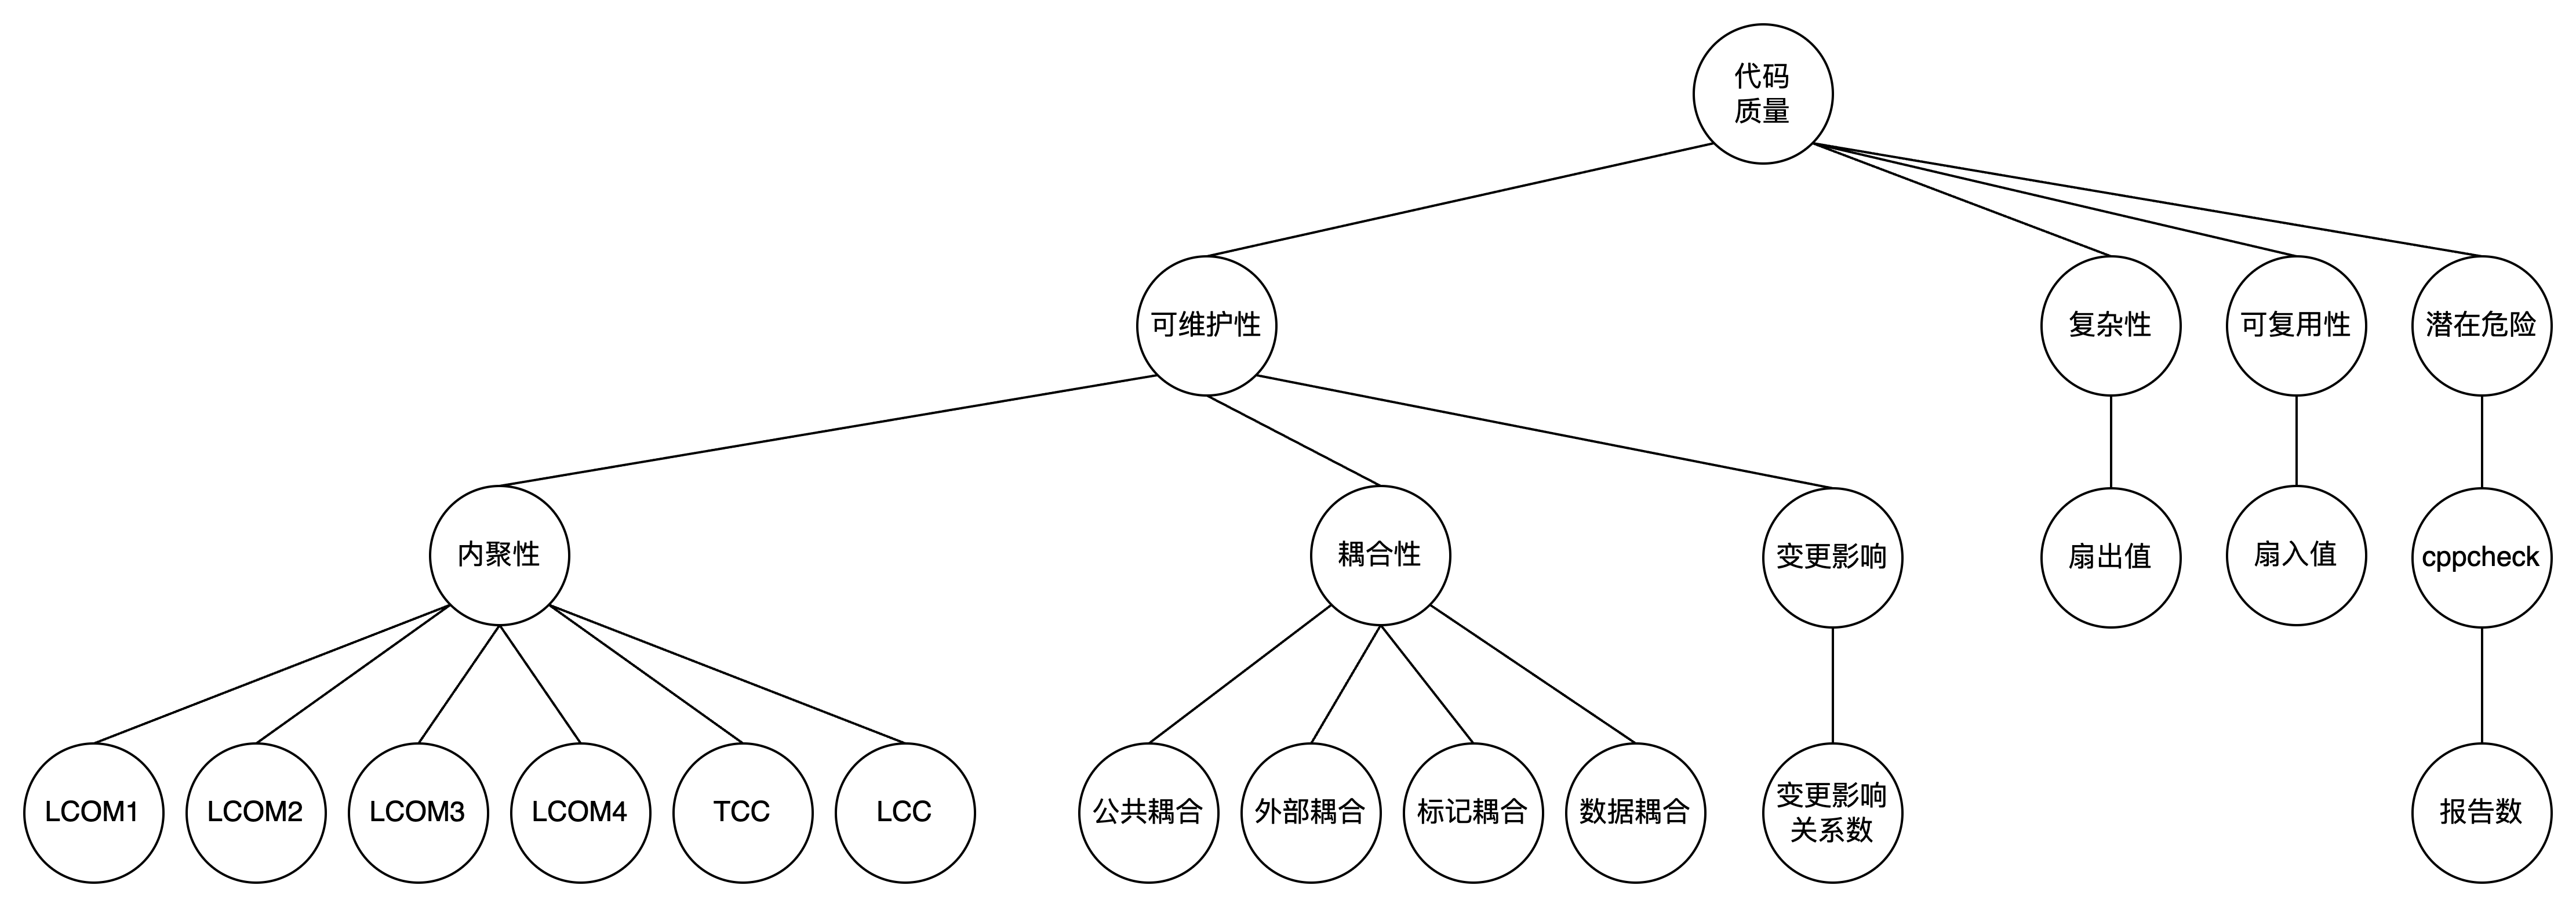
\includegraphics[width = 1.0\textwidth]{质量模型.jpg}
\caption{代码质量度量模型}
\end{figure}

在对代码质量的的评价上,我们的分为模块级和方法级的两个层次的度量,其中内聚性为模块级度量,其他度量为方法级。通常评价可分为绝对评价和相对评价两种,对于一组相同设计目的代码,相对评价更为合适\cite{黄沛杰2011代码质量静态度量的研究与应用},一个项目内的模块或方法可以看作设计目的相同的代码,方便用户在项目中关注到相对来说质量较差的代码。

\paragraph{度量元度量} 使用统计中常用的分档方式,分五个档次对应优、良、中、低、差,按式的方式给定参考分值。对于度量值越小越好的度量元,假设代码$c$的质量属性$k$中子属性$i$度量元$j$对应的最大值和最小值分别是$\max_{ij}$和$\min_{ij}$,测试值区间 \(Z_{ij}\) 和测试值 \(t_{ij}\) 在 \(Z_{ij}\) 中的位置 \(t'_{ij}\) 分别为:
\begin{align}
Z_{ij} = \max_{ij} - \min_{ij}
\end{align}
\begin{align}
t'_{ij} = t_{ij} - \min_{ij}
\end{align}

相对评价的分值 \(V_{ij}^k\) 如式。
\begin{align}
V_{ij}^c = 
\begin{cases} 
100, & t'_{ij} \leq 0.2Z_{ij} \\ 
80, & 0.2Z_{ij} < t'_{ij} \leq 0.4Z_{ij} \\ 
60, & 0.4Z_{ij} < t'_{ij} \leq 0.6Z_{ij} \\ 
40, & 0.6Z_{ij} < t'_{ij} \leq 0.8Z_{ij} \\ 
20, & 0.8Z_{ij} < t'_{ij}
\end{cases}
\end{align}

对于度量值越大越好的度量元,只需把式中分值倒序。

\paragraph{质量子属性度量} 一个质量子属性包含一个或多个度量元。在这里将一个子属性下的所有度量元进行组合,总的评估质量子属性。定义代码c的子属性度量$U_{i}^c$ 如式(),这里将各度量元的权重设为等值。

\begin{align}
U_i^c = \sum_j w_{ij} V_{ij}^c, \quad \sum_j w_{ij} = 1
\end{align}

\paragraph{质量属性度量} 通过对质量特性下的度量元进行运算得到代码质量特性的度量,计算公式如下,这里将各子属性的权重设为等值。质量特性度量可以作为代码在某一方面的质量表现情况,在实际情况下可以单独使用,因此这里不再对质量特性度量进行聚合评分。

\begin{align}
Q_k^c = \sum_i w_{ki} U_{i}^c, \quad \sum_i w_{ki} = 1
\end{align}

\subsection{基于内聚度缺乏度和连通性的的内聚性度量}

\paragraph{基于内聚度缺乏度的内聚度计算} LCOM(Lack of Cohesion in Methods)系列指标是根据模块内聚度的缺乏程度来衡量模块的内聚度的指标。在本文中,
面向对象语言以类为研究范围进行计算内聚度,非面向对象的语言以文件为研究范围进行计算,类中的成员属性对应文件中的全局变量,类中的成员方法对应文件中定义的方法。LCOM 指标的核心思想是度量一个类中方法
对实例变量(属性)的共享程度。不同版本的 LCOM 有着不同的计算方法和含义,体现了不同的侧重点。这里一共计算以下四个指标,

(1)LCOM1,含义是不引用相同字段的方法对数目\cite{1994Ametr}。计算公式如式(2-1)。
\begin{equation}
LCOM1 = C_{n}^{2}-e
\end{equation}

其中n 是文件中的方法总数,e 是引用相同字段的方法对。以图2-4为例介绍计算方式,其中椭圆表示方法,点表示变量,点在椭圆内表示该方法引用了该变量。LCOM1值为\(C_{6}^{2} - 5 = 10\)。

\begin{figure}[h]
\centering
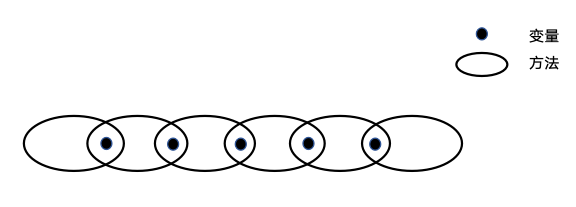
\includegraphics[width = 0.7\textwidth]{内聚度示例.jpg}
\caption{示例模块}
\end{figure}
    

(2)LCOM2,含义是不引用相同字段方法对与引用相同字段方法对数之差\cite{1996Coupling}。其计算公式如式(2-2)。

\begin{equation}
    {LCOM2}=\left\{
        \begin{array}
        {c}P-Q,  ifP\geq Q \\
        0,  otherwise
        \end{array}\right.
\end{equation}

其中,P 是不共享实例变量的方法对的数量,Q 是共享实例变量的方法对的数量。
如果 LCOM1 的结果为负数,则被置为 0。图2-4模块中,不共享变量的方法对P为10,共享变量的方法对Q为5,LCOM2值为P-Q=5。

(3)LCOM3是对前两种指标的进一步改进,其计算公式如式(2-3):
\begin{equation}
LCOM3 = \frac{\left( \frac{1}{a} \sum_{j=1}^a \mu(A_j) \right) - m}{1 - m}
\end{equation}

其中\( m\)为文件中的方法数,\( a\)表示文件中的变量数,\( mu(A_j)\)表示的是引用变量\(A_j\)的方法数。如图2-5所示的文件中有3个方法和3个变量,计算方式如图所示。
\begin{figure}[h]
\centering
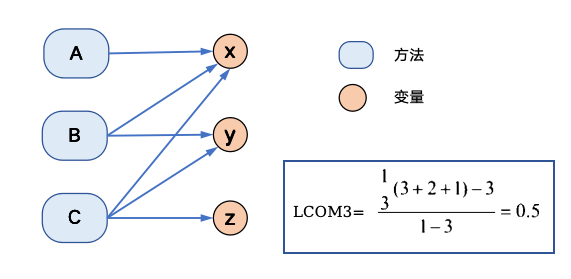
\includegraphics[width = 0.7\textwidth]{LCOM3.jpg}
\caption{LCOM3计算示例}
\end{figure}



(4)LCOM4,含义是以方法和变量为顶点,方法引用字段或方法之间有调用关系则两节点之间有条边构成图的连通分支数\cite{1995Measuring}。计算时,根据深度优先搜索的方式,计算图中的连通分支数,得到的值即为LCOM4。如图2-6所示的两个文件的LCOM4的值分别为2和1。

\begin{figure}[h]
\centering
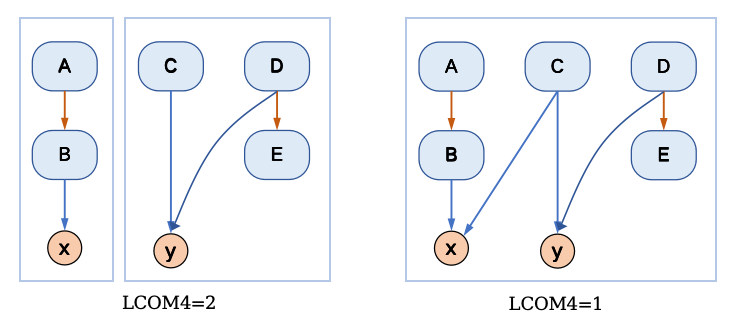
\includegraphics[width = 0.7\textwidth]{LCOM4.jpg}
\caption{LCOM4计算示例}
\end{figure}


\paragraph{基于连通性的内聚度计算} TCC(Tight Class Cohesion)和 LCC(Loose Class Cohesion)是用于衡量模块内
聚度的指标,这两个指标主要关注于模块中方法之间的连通关系,核心思想是通过
分析模块中方法如何相互作用以及如何访问共同资源(如全局变量)来评估模块的内聚度。

(1)TCC,含义是有连通关系的方法对数与总方法对数的比值\cite{1995Cohesion}。
TCC 关注于模块中方法之间的“直接连接”。如果两个方法直接共享访问同一个变
量,则认为这两个方法是直接连接的。计算公式如式(2-4)。
\begin{equation}
{TCC} = \frac{e}{C_{n}^{2}}
\end{equation}

其中\(n\)是文件中的方法总数,\(e\)是图中的直接连接边数。

(2)LCC则基于方法间接引用共同字段的关系进行计算\cite{1995Cohesion}。
LCC 除了考虑直接连接的方法对外,还包括了间接连接的方法对。如果两个方法不
是直接连接,但可以通过一系列的方法调用或变量引用来连接,则认为它们是间接连接的。LCC 的值基于模块中直接或间接连接的方法对占所有可能方法对的比例来计算。因此,LCC 的值通常不低于 TCC 的值,并且提供了一个更宽泛的模块内聚度视角。计算公式如式 (2-5):
\begin{equation}
{LCC=\frac{e+e_{indirect}}{C_{n}^{2}}}
\end{equation}

其中\(n\)是文件中的方法总数,\(e\)是图中的直接连接边,\(e_{indirect}\)是除直接连接边的边数。如图2-7是计算LCC和TCC的例子,左图中通过方法AB通过变量x直接连接,方法CD通过变量y直接连接,直接连接和间接连接都是2。而右图中直接连接是AB、BC、BC和CD,间接连接是AD和BD,因此计算结果如图。

\begin{figure}[h]
\centering
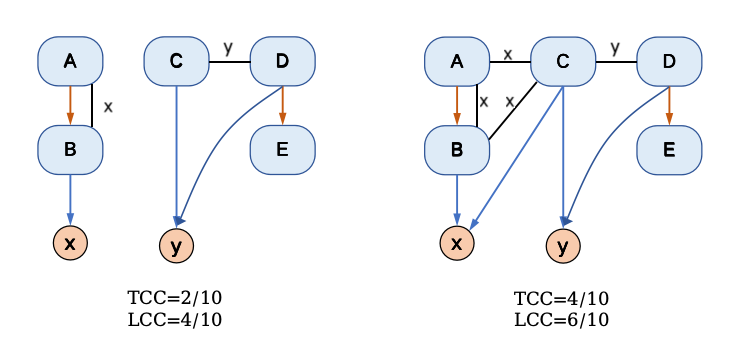
\includegraphics[width = 0.7\textwidth]{TCCLCC.jpg}
\caption{TCC和LCC计算示例}
\end{figure}


\subsection{方法间耦合性度量}

耦合是在软件架构中用来描述模块间相互依赖和连接程度的一个重要指标。耦合度的高低直接影响到系统的维护性和可扩展性。在现有的研究和实践中,耦合度通常被细分为六个等级,如表2-1所示,这些等级从高到低反映了模块间依赖的紧密程度。本文关注的是方法与方法之间的耦合性。通过深入分析方法级别的耦合性,研究方法如何通过参数传递、调用关系、共享全局变量等方式相互依赖,我们可以更准确地识别潜在的设计缺陷和优化机会,从而提高系统的模块化程度,增强系统的可维护性和可扩展性。

\begin{table}[htbp]
\caption{软件架构中耦合性分类}
\vspace{0.5em}\centering\wuhao
\begin{tabular}{ccccc}
\toprule
耦合性类别 & 描述 & 耦合程度 & 本文是否分析 \\
\midrule
内容耦合 & 模块直接访问或修改另一个模块的内部数据 & 6 & 否\\
公共耦合 & 模块访问同一公共数据环境 & 5 & 是 \\
外部耦合 & 模块共享全局简单数据结构 & 4 & 是 \\
控制耦合 & 模块传递控制信息,影响计算流程 & 3 & 否 \\
标记耦合 & 通过参数传递复杂数据结构信息 & 2 & 是 \\
数据耦合 & 通过参数传递简单数据 & 1 & 是 \\
\bottomrule
\end{tabular}
\end{table}


内容耦合是耦合度最高的一种形式,它表示一个模块能够直接访问或修改另一个模块的内部数据和结构。在方法级的耦合分析中,这种耦合形式通常不被考虑,因为方法间的直接数据访问往往通过参数传递或者 API 调用实现,而不是直接的内容访问。

公共耦合发生在多个模块共同访问某个全局数据环境时。这种数据环境可能是全局数据结构、全局变量或内存公共区域等。在提取到的全局变量表中,对于复杂数据结构如结构体和数组,其引用点所在的方法之间均存在公共耦合关系。


外部耦合与公共耦合相似,但区别在于它涉及的是对全局简单变量的访问。例如,当多个模块访问或修改相同的全局简单类型变量时,则这些模块之间存在外部耦合。


控制耦合指模块之间传递信息中包含用于控制模块内部的信息。在提取到的方法摘
要表中,遍历方法,如果该方法调用其他方法时,对应方法的参数列表中有变量决定了被调用方法中的计算流程,则方法之间存在控制耦合关系。由于本文不考虑分析方法内部的控制逻辑,因此不提取此种耦合。


标记耦合指通过参数表传递数据结构信息,调用时传递的是数据结构。在方法摘要
表中提取了方法的参数列表,包括参数名和参数类型,根据参数类型,可以确定
参数表中是否包含复杂类型。除此之外,在方法的调用表中,也提取了方法调用的
其他方法,结合这两个信息,即可确定两个方法是否存在着标记耦合关系。


数据耦合指通过参数表传递简单数据。与标记耦合类似,根据参数类型可以确定参
数是否全部为基本类型,结合方法调用表,即可确定两个方法是否存在数据耦合。

\subsection{方法扇入扇出度量}

方法的扇入(Fan-in)和扇出(Fan-out)是软件工程中常用于衡量方法可复用性和方法复杂性的两个指标。

\begin{figure}[h]
\centering
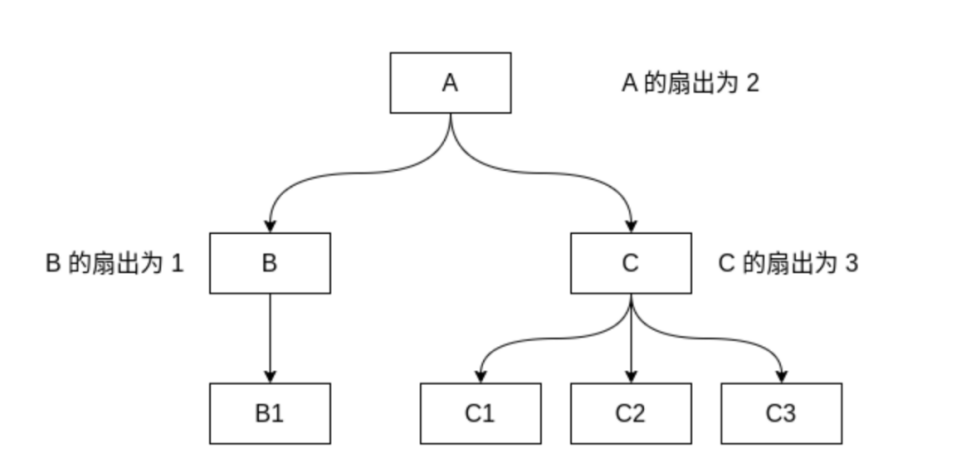
\includegraphics[width = 0.8\textwidth]{扇入扇出.png}
\caption{扇入扇出实例}
\end{figure}

扇入是指调用某个方法的不同方法的数量。扇入值较高的方法通常被认为是重要的或核心的,因为它们被多个其他方法所依赖。高扇入值可能意味着该方法执行了一个基础或共享的任务。可复用性较强。


扇出是指某个方法直接调用的不同方法的数量。它表示了一个方法对其他方法的影
响程度。扇出值较高的方法可能更复杂,因为它们需要管理和协调更多的方法调用。高扇出值可能意味着该方法具有较高的责任度,且可能更难以理解和维护。


本文中对于提取到的方法摘要表,遍历每一个方法,统计其调用方法的数量即可计算出该方法的扇出值,再以该方法名在方法摘要表中搜索调用了该方法的方法,统计总数,得到的值即为扇入值。

\subsection{基于静态检测工具的潜在缺陷度量}

为了更准确地计算潜在危险度量,本文结合了静态代码分析工具 Cppcheck,对项目中的源代码进行检测和分析。Cppcheck 是一款开源的静态分析工具,专门用于检测 C/C++ 代码中的潜在错误和编码规范问题。Cppcheck会根据问题的严重性和类别将检测出的问题如表2-2所示的六类。

\begin{table}[htbp]
\caption{cppcheck报告问题分类}
\vspace{0.5em}\centering\wuhao
\begin{tabular}{cccc}
\toprule
类别 & 描述 \\
\midrule
error &  严重错误 \\
warning & 潜在的错误或不推荐的做法 \\
style & 代码风格问题,通常与代码格式、命名约定等相关 \\
performance & 性能问题,表明当前方式可能效率不高 \\ 
portability & 平台相关问题,可能导致在不同环境出现不同行为 \\
information & 额外的信息或建议 \\ 
\bottomrule
\end{tabular}
\end{table}

检测结果中包括了诸如错误、警告和代码风格问题等不同级别的信息,这些信息帮助开发者识别代码中的潜在问题。

Cppcheck 提供的报告与其他度量指标相结合,共同构成了全面的质量评估体系。用户可以根据检测报告对代码质量进行更细致的判断和分析,从而为后续的优化和重构提供科学依据。通过这种方式,本研究实现了对代码质量的多维度综合评价,为开发者提供了更为精确的质量检测和改进方向。



\section{代码审查图的构建和代码结构的可视化}

\subsection{代码审查图构建}

为帮助用户从宏观的角度了解项目结构和代码质量,本章提出一种名为代码审查图的可视化方式。代码审查图主要由两个核心元素构成,分别是节点和边。其中,节点代表软件项目中的方法或全局变量,边表示节点之间的各种关系,包括耦合关系、变更影响关系以及依赖调用关系。这些元素的结合能够帮助开发者从全局视角理解和评估项目的结构和质量,尤其是在进行代码审查和代码变更时。

\paragraph{节点构建} 节点的作用是标识项目中的方法和全局变量。通过前文所述的方法摘要表和全局变量信息表,我们为每个方法和全局变量创建了对应的节点。每个节点都具有多个属性,这些属性能够提供有关节点所代表的方法或变量的关键信息,便于开发者对代码进行全面的审查和分析。



方法属性分为两个主要部分:首先是方法的基本信息,如表4-1所示。

\begin{table}[htbp]
\caption{代码审查图节点属性-基本信息}
\vspace{0.5em}\centering\wuhao
\begin{tabular}{cccc}
\toprule
    属性 & 描述 \\
\midrule
方法名 & 方法名,由方法所在路径和方法名拼接而成,保证唯一  \\
方法参数 & 方法的参数列表,包括参数的名称和类型   \\
方法内调用方法 & 本方法内调用的其他方法名   \\
方法可作用域 & 表明方法是否全局可用   \\
方法所在模块 &  方法所在模块,目前表示为方法所在文件  \\ 
\bottomrule
\end{tabular}
\end{table}

这一部分包括方法的名称、所在模块、方法签名、访问修饰符等,这些属性有助于开发者了解方法的基本信息。例如,方法的名称可以反映其业务功能,所在模块和作用域则有助于理解方法的上下文和调用约束等。

其次是与代码质量相关的度量和信息,如表4-2所示。

\begin{table}[htbp]
    \caption{代码审查图节点属性-质量相关信息}
    \vspace{0.5em}\centering\wuhao
    \begin{tabular}{ccp{5cm}p{5cm}}
    \toprule
    质量属性& 质量子属性 & 度量元 & 描述 \\
    \midrule
    
    \multirow{3}{*}{可维护性} 
    & 内聚性& LCOM1、LCOM2、LCOM3、LCOM4、TCC、LCC &  总的相对评分、相应建议、具体的属性值 \\           
    & 耦合性& 数据、标记、外部、公共耦合数 &  总的相对评分、建议、与本方法存在数据、标记、外部、公共耦合关系的方法 \\       
    & 变更影响 & 变更影响关系数 & 总的相对评分、与本方法存在变更影响的方法 \\  \cline{2-4}
    复杂性 & 扇出 &扇出值 &  总的相对评分、建议、方法的扇出值 \\  \cline{2-4}
    重用性 & 扇入 &扇入值 &  总的相对评分、建议、方法的扇入值 \\  \cline{2-4}
    潜在危险 & 静态代码缺陷 & 缺陷数 &  总的相对评分、cppcheck检测得到的本方法缺陷信息 \\      
    \bottomrule
    \end{tabular}
    \end{table}

这一部分将展示前文根据质量度量模型得到的代码的4种质量属性情况,包括可维护性、复杂性、重用性和潜在危险四个方面,并且将这四个方面的特性根据度量进行分档,给出分档等级。同时为了进一步指导用户对具体质量子属性进行优化,还报告了质量子属性的相对质量情况,对于较差的子属性向开发者提供有针对性的改进建议。例如,如果某个方法的扇出度较差,则可能表明该方法在项目中的依赖关系过于复杂,可能需要拆分。类似地,如果某模块的内聚性较差,则说明模块内部各元素的依赖关系较为松散,指导用户对该模块进行重构。

对于全局变量的属性则主要包含表4-3中的信息。主要是对全局变量基本信息的展示,方便开发者快速了解该变量的作用域、使用情况以及与其他代码部分的关联性。通过这些信息,开发者能够更好地理解变量在整个项目中的作用以及对应的代码上下文。

\begin{table}[htbp]
\caption{代码审查图节点属性-全局变量信息}
\vspace{0.5em}\centering\wuhao
\begin{tabular}{cccc}
\toprule
    属性 & 描述 \\
\midrule
变量名 & 全局变量名,由所在路径和变量名拼接而成,保证唯一  \\
变量类型 & 变量类型   \\
被使用方法 & 使用了本全局变量的方法名   \\
变量可使用域 & 表明变量是否全局可用   \\
方法所在模块 &  变量所在模块,目前表示为所在文件  \\  
\bottomrule
\end{tabular}
\end{table}


\paragraph{边的设计}

在代码审查图中,边表示节点与节点之间的关系,这些关系揭示了软件系统中各个方法与全局变量之间的相互依赖和影响。根据其性质,边的类型主要分为三类,具体分类如表4-4所示:静态依赖关系、耦合关系和变更影响关系。

其中静态依赖关系分为方法之间的调用关系和方法与全局变量的引用,耦合关系如表4-2中所示共4类,变更影响关系则是根据第三章方法检测得到的变更影响关系。

每种关系反映了不同层次的代码相互作用,帮助开发者全面理解系统的结构和潜在的质量风险。

\begin{table}[htbp]
\caption{代码审查图边分类}
\vspace{0.5em}\centering\wuhao
\begin{tabular}{cccc}
\toprule
属性 & 描述 \\
\midrule
静态依赖关系 & 含方法之间调用、方法引用全局变量两种  \\
耦合关系 & 含数据耦合,标记耦合,外部耦合,公共耦合四种   \\
变更影响关系 & 由第三章方法检测得到  \\
\bottomrule
\end{tabular}
\end{table}



\subsection{代码审查图可视化}

本节从代码审查图的可视化方案和交互方案两个方面展开介绍。

\paragraph{可视化方案}

代码审查图的可视化方案基于开源项目 G6。G6 是一个强大的图形可视化引擎,提供了绘制、布局、分析、交互、动画等全方位的图形可视化基础功能,具有简单易用且完备的特性。G6 具有两个显著优势。

(1)数据与可视化图形分离:在使用 G6 时,用户只需将图的数据组织为 JSON 格式,如图4-3所示,包括节点信息和边信息,直接传递给 G6 即可自动生成对应的力导向图。这种数据与图形的分离不仅简化了开发流程,还提高了数据的灵活性和可操作性,便于进行后续的数据更新和图形重绘。

\begin{figure}[h]
\centering
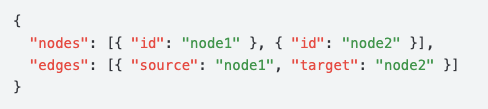
\includegraphics[width = 0.6\textwidth]{G6图数据示例.jpg}
\caption{G6图数据示例}
\end{figure}

(2)高度的定制能力:G6 提供了丰富的图形展示配置选项,用户可以根据需求自由选择不同的样式和布局方式。如果 G6 内置的元素不满足特定需求,它还支持用户自定义节点、边及其他元素,使得图形展示更加贴合实际应用场景。

本文使用G6内置节点和边实现代码审查图的可视化。G6的节点构成共包含6部分,其中label表示文本标签,通常用于展示节点的名称或描述,本文中将节点属性赋值给label,便于用户查看属性相关信息。G6的边的构成共包含4部分,label具有同样的功能,将边的类别用于label。让 G6 加载此数据源进行展示,就实现了同时也实现了计算逻辑与图形可视化的有效分离。


\paragraph{交互方案}

对于软件项目这样的分析对象,方法和全局变量的数量常达到千级别,对于一个图来讲,这样的级别很难在图中展示完所有的信息,因此需要用户交互,来展示更详细的信息。表4-5展示了目前代码审查图的交互和对应的逻辑设计。


\begin{table}[htbp]
\caption{代码审查图交互和逻辑设计}
\vspace{0.5em}\centering\wuhao
\begin{tabular}{cccc}
\toprule
交互方式 & 业务逻辑 \\
\midrule
视角缩放 & 操作鼠标滚轮对图进行缩放  \\
视角移动 & 鼠标拖拽移动整个代码审查图   \\
聚焦节点 & 光标悬停在节点上显示节点的方法名/变量名  \\
移动节点 & 鼠标长按节点拖拽可移动节点 \\
查看节点属性 & 鼠标点击节点展开节点属性  \\
聚焦关系 & 光标悬停在边上显示边的类型  \\
查看关系信息 & 鼠标点击节点展开节点属性  \\
节点筛选 & 通过点击筛选节点按钮,确认是否筛选掉孤立节点 \\
\bottomrule
\end{tabular}
\end{table}


\section{基于代码审查图的代码质量分析}


代码审查图能直观体现模块或方法层面上与代码质量相关的特征,从而辅助用户理解代码质量较差或较好的具体原因。本节通过分析项目代码历史版本中被修复或重构的代码对应的代码审查图结构,总结了以下5种不良的图模式。它们在不同的角度上反映了代码较差的质量属性和对应的优化方向。

\paragraph{冗余代码元素} 冗余代码元素指的是在代码中定义但从未被使用的代码元素。在代码审查图中表现为孤立节点,如图\ref{1_冗余代码图模式}所示。即某个节点不与任何其他节点存在边的图模式。这意味着该代码元素不和任何其他代码产生依赖、调用等联系,不论是作为全局变量还是方法出现,都会消耗不必要的性能和资源,且影响其所在模块的内聚程度。优化时,可以考虑去掉冗余代码,只保留和软件核心逻辑相关的代码。

\begin{figure}[h]
\centering
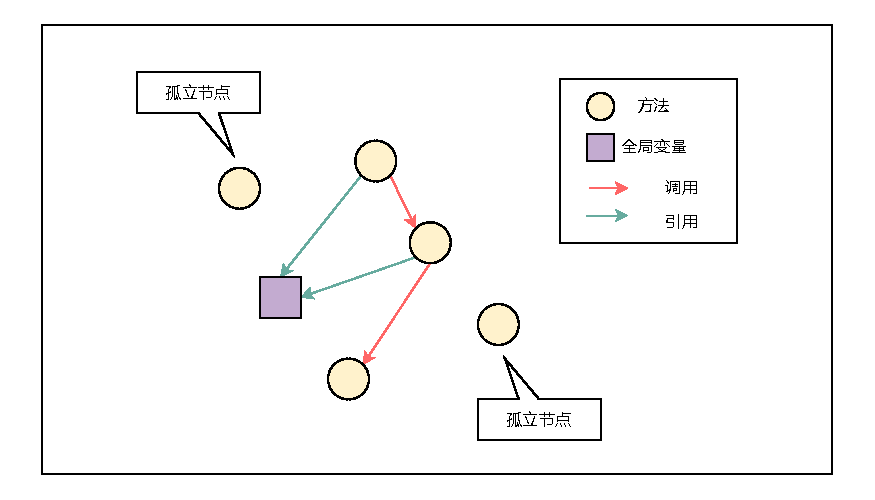
\includegraphics[width = 0.6\textwidth]{孤立节点图模式.pdf}
\caption{冗余代码图模式}
\label{1_冗余代码图模式}
\end{figure}



\paragraph{长嵌套调用} 长嵌套调用在代码审查图中的表现方式是方法间的链式连接,如图\ref{1_长嵌套调用图模式}所示。长嵌套调用有以下几点危害,1.可读性差:层次过多的嵌套调用会使代码结构变得复杂,理解代码的执行顺序和逻辑变得困难。2.可维护性差:由于链式的松散结构,模块的可维护性也会变差,当需要对中间环节进行变更时,可能会影响整个嵌套调用的逻辑。3.性能问题:方法调用会涉及到栈帧的创建和销毁,长的嵌套调用会导致栈的深度增加,频繁的栈操作可能会影响性能。在代码审查图中可以直观地发现嵌套调用的现象。优化时可以考虑合并部分底层方法,减少嵌套层数来优化代码。

\begin{figure}[h]
\centering
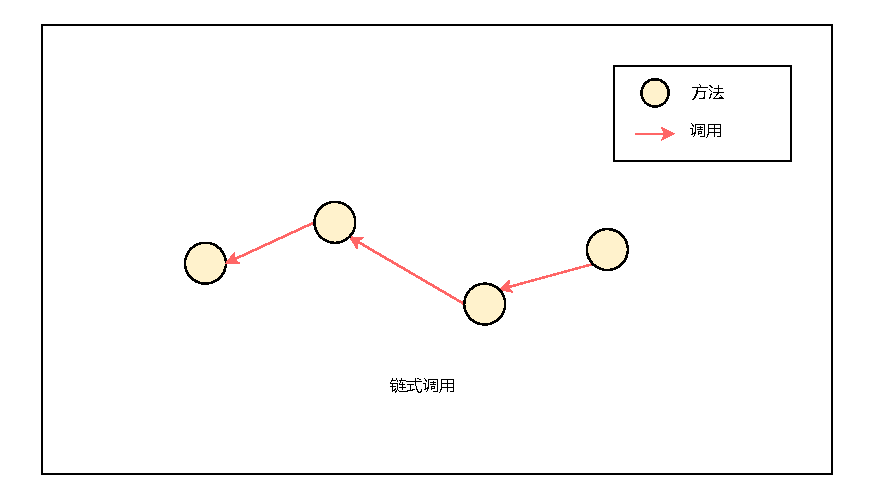
\includegraphics[width = 0.6\textwidth]{链式调用模式图.pdf}
\caption{长嵌套调用图模式}
\label{1_长嵌套调用图模式}
\end{figure}




\paragraph{复杂方法} 复杂方法的特性之一是职责过多,通常表现为方法内部调用了过多的其他方法或与大量方法存在变更影响关系,这种特征在代码审查图中表现为具有大量的出边的中心化节点,如图\ref{1_复杂方法图模式}所示。这种方法的危害有以下几点,1.可维护性差:依赖过多外部方法,任何外部方法的变动都可能导致当前方法的变动,增加维护成本。2.增加耦合度,降低了系统的灵活性。3.违背单一职责原则。

\begin{figure}[h]
\centering
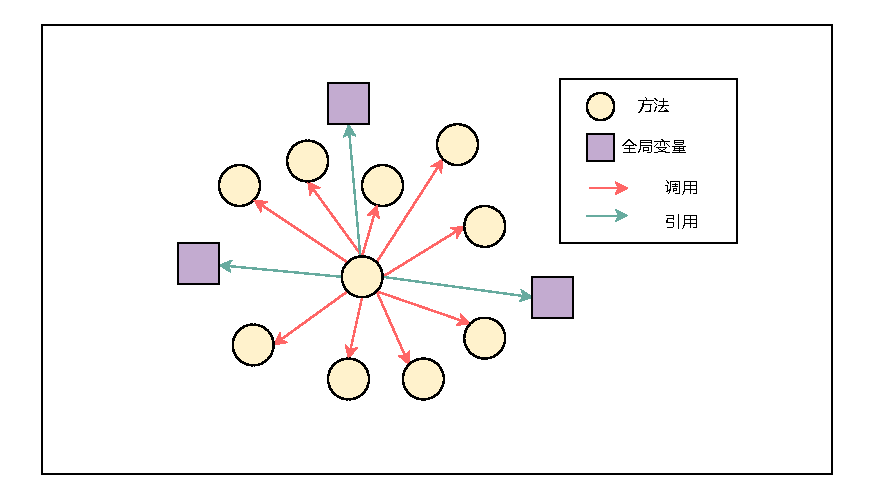
\includegraphics[width = 0.6\textwidth]{复杂方法.pdf}
\caption{复杂方法图模式}
\label{1_复杂方法图模式}
\end{figure}



通过代码审查图用户可以迅速定位到复杂方法,深入了解其上下文信息,进而判断其是否存在不合理的复杂度。优化时,用户可以考虑分解为小函数等方式重构该方法、简化其职责并调整其与其他模块的关系,从而有效提升系统的可维护性和可扩展性。


\paragraph{职责不匹配} 在软件项目里,每个代码元素都处于特定的物理位置,比如所在的文件、类、文件夹等。这种物理位置往往体现了软件最初的设计理念。而在静态代码结构中,每个代码元素还处于特定的逻辑位置,这在代码审查图中,表现为与其他代码元素的相对位置关系。对于某些方法而言,会出现一种情况:其承担的职责与它所处的物理位置不再完全适配,反而与其他模块的关联更为紧密。我们将这种问题称作职责不匹配问题。

\begin{figure}[h]
\centering
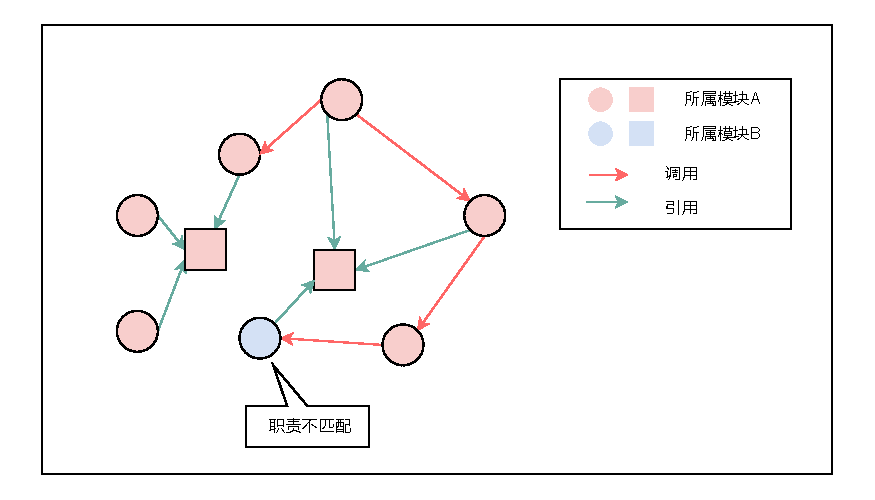
\includegraphics[width = 0.6\textwidth]{figures/职责不匹配.pdf}
\caption{职责不匹配图模式}
\label{1_职责不匹配图模式}
\end{figure}

代码审查图中,相同模块的代码元素呈现为同一颜色,不同模块不同颜色,得益于力导向的可视化特性,逻辑上紧密依赖的节点聚集在一起。职责不匹配的特征在代码审查图中的模式如图\ref{1_职责不匹配图模式}所示,表现为逻辑聚集的节点颜色不统一,某些节点(如图\ref{1_职责不匹配图模式}中的蓝色节点)与模块的主色调(红色节点)不符。优化时一般有两种角度,如果用户认可最初的设计理念,可将职责不匹配的代码与主模块进行拆分,如果用户认为逻辑位置更为合适,则可将职责不匹配的代码合并进主模块。通过这样的重构操作,可将依赖和变更影响关系限制在同一模块内,避免变更时跨模块的影响。


\paragraph{模块间不良的逻辑型变更影响} 对于软件代码而言,模块间的变更影响关系应当以依赖型变更显式地呈现,这有助于开发者在静态结构中清晰地识别依赖关系。相比之下,逻辑型变更影响往往隐匿在代码内部,仅通过代码上下文或前后调用关系难以察觉。模块间的变更影响通常被视为不利因素,它可能导致不良变更传播问题。

\begin{figure}[h]
\centering
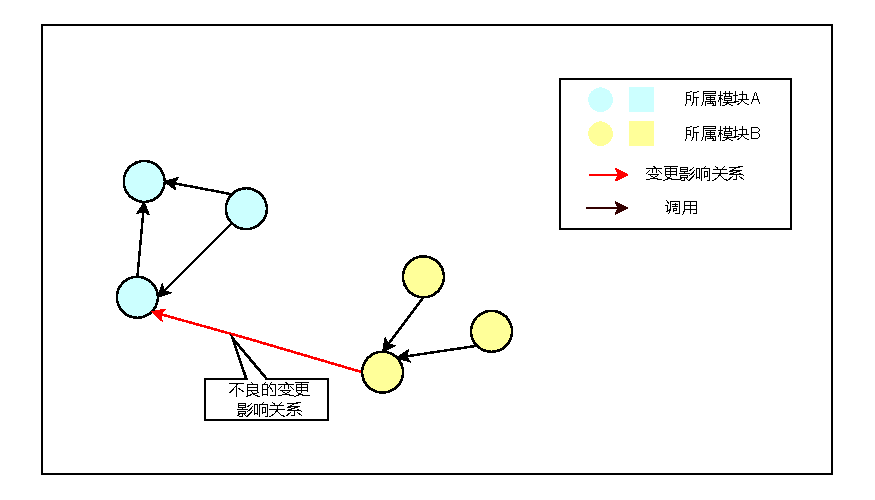
\includegraphics[width = 0.6\textwidth]{figures/不良变更影响.pdf}
\caption{不良的逻辑型变更影响}
\label{1_不良的逻辑型变更影响}
\end{figure}


这种不良的逻辑型变更影响在代码审查图中表现为图\ref{1_不良的逻辑型变更影响}所示的模式,其中红色边表示逻辑型变更影响关系,黑色边表示由调用引起的依赖型变更影响关系。两个模块由于逻辑型影响被连接在一起,导致变更时很难察觉,且模块间互相影响。这种现象暴露了系统架构中的潜在问题——虽然各模块内部结构较为合理,但模块间的依赖关系复杂且紧密,增加了维护和变更时的复杂性与风险。为了解决这一问题,优化的建议是尽量减少或消除这些不良的变更影响关系,或者将其转化为依赖型影响,从而减少隐匿的跨模块变更传播的可能性。




% \section{代码质量评估报告生成}

% 在软件开发和代码审查的过程中,开发者通常可以借助代码审查图聚焦于代码的上下文,帮助发现局部代码的问题。然而,当软件开发完成,开发者希望从全局角度对软件项目的整体质量进行衡量时,仅依靠代码审查图可能会存在质量信息过于分散、不易聚焦的问题。因此,本节进一步通过生成文档化的代码审查报告,为开发者提供统一的代码质量概览,帮助其全面掌握项目的质量状况。

% 代码审查报告的核心目标是揭示软件项目中存在的关键质量问题,并以本文提取的代码质量属性与子属性为主线,系统性地向用户报告代码中的相对质量子属性为差的模块或方法,并给出相应的建议。

% 为了帮助用户在代码开发过程中防止变更不完全,报告还将列出项目中所有的代码变更影响关系。用户可以参考这些信息,在变更时全面评估影响范围,降低遗漏风险。

% 通过对这些信息的整合与分析,生成的报告文档为用户提供了一份全面的代码质量概览,既可以帮助用户识别代码中的潜在问题,又能为系统的后续优化与维护提供指导性建议。

\section{实验结果与分析}

\subsection{实验设计和实验数据}

 为了验证所提的代码度量模型与基于代码审查图的质量分析的有效性,本实验从软件的历史版本变更角度出发,结合代码度量和图模式,探讨修复和重构概率大的代码与其质量之间的关系,从而验证其有效性。

\paragraph{验证代码质量度量模型的实验设计}  本实验的核心数据是代码历史版本和对应的提交记录,具体步骤如下:

\noindent 1. 代码历史版本收集。将代码历史提交按以下原则进行筛选,筛选后收集提交前版本的项目源代码,提取该提交变更的方法,得到<code,list<changed\_func>>的二元组。

\begin{itemize}
    \item 按关键词筛选提交:保留提交信息中包含以下关键词的提交:\{ fix, refactor, Fix, Refactor \}。这些关键词通常出现在与缺陷修复和代码重构相关的提交中,能够反映用户提高代码质量的操作。
    \item 按代码差异类型筛选:进一步分析代码差异,判断是否涉及修复或重构。
\end{itemize}

\noindent 2.对于每一个提交,对提交前版本的项目源代码进行代码度量计算,不同的质量属性内部进行分档排名,得到方法之间的相对质量关系。

\noindent 3.将该提交的提交变更方法与不同分档进行求交集,得到每档中方法变更的数量。

\noindent 4.观察代码质量度量和变更概率的数量关系,验证有效性。

\paragraph{验证代码审查图的实验设计} 

与前述步骤相似,先对提交进行筛选并收集提交前代码版本。对变更前的版本进行代码审查图生成,对于变更部分识别其是否具有不良图模式。


\paragraph{实验数据} 本章选取jemalloc为示例项目进行验证。

\begin{table}[htbp]
\caption{jemalloc数据统计}
\vspace{0.5em}\centering\wuhao
\begin{tabular}{cccccc}
\toprule
项目属性 & 数值/信息 \\
\midrule
总提交 & 3530 \\
包含修复提交 & 653  \\
包含重构提交 & 53  \\
修复提交抽样 & 10 \\
重构提交抽样 &  10 \\
\bottomrule
\end{tabular}
\end{table}


\subsection{实验环境}

(1)实验环境

实验环境如表4-6所示。

\begin{table}[htbp]
\caption{实验环境}
\vspace{0.5em}\centering\wuhao
\begin{tabular}{cccc}
\toprule
    环境 & 信息 \\
\midrule
操作系统 & macOS Ventura v13.5.2  \\
python & 3.7   \\
Java & 1.8   \\
G6 & g6.min.js 4.3.11  \\  
libclang & 15.0.7  \\ 
pycparser & 2.21  \\
\bottomrule
\end{tabular}
\end{table}


% 对于代码审查报告的生成,则是验证审查报告的格式是否符合设计方案。

\subsection{实验结果分析}

RQ1: 代码质量度量模型能否有效反映项目的质量情况?在修复或重构过程中,代码质量如何影响开发人员的修改决策?

RQ2: 基于代码审查图分析得到的不良质量信息是否真实,代码审查图中能反映哪些不良的代码模式?


\textbf{1.针对于RQ1的实验}

% jemalloc
% 文件206个
% 方法2001个

实验结果如表所示

通过表可以看出,在修复或重构等操作过程中,大多数变更都集中在代码质量较差的部分。这表明,质量较差的代码相较于质量较好的代码,在重构或修复的提交中更容易被修改。这一现象进一步验证了代码质量模型的有效性,它能够在项目中识别出质量较差的代码区域,从而帮助开发人员优先关注这些部分,在提升整体代码质量时有针对性地进行优化和重构。因此,代码质量模型不仅提供了对现有代码质量的量化评估,还能为项目团队提供具体的优化方向,确保资源投入最大化地改善代码质量。

\textbf{2.针对于RQ2的实验}

针对4.4节总结的不良的图模式,在示例项目中均有对应模式的代码审查图子图。这里以TheAlgorithms项目和jemmaloc项目中实际出现过,后又被重构行为变更了的子图为例,说明了代码审查图可以帮助用户发现此类不良的代码结构。

\begin{figure}[!h]
    \setlength{\subfigcapskip}{-1bp}
    \centering
    \begin{minipage}{\textwidth}
    \centering
    \subfigure[antiword-未划分模块]{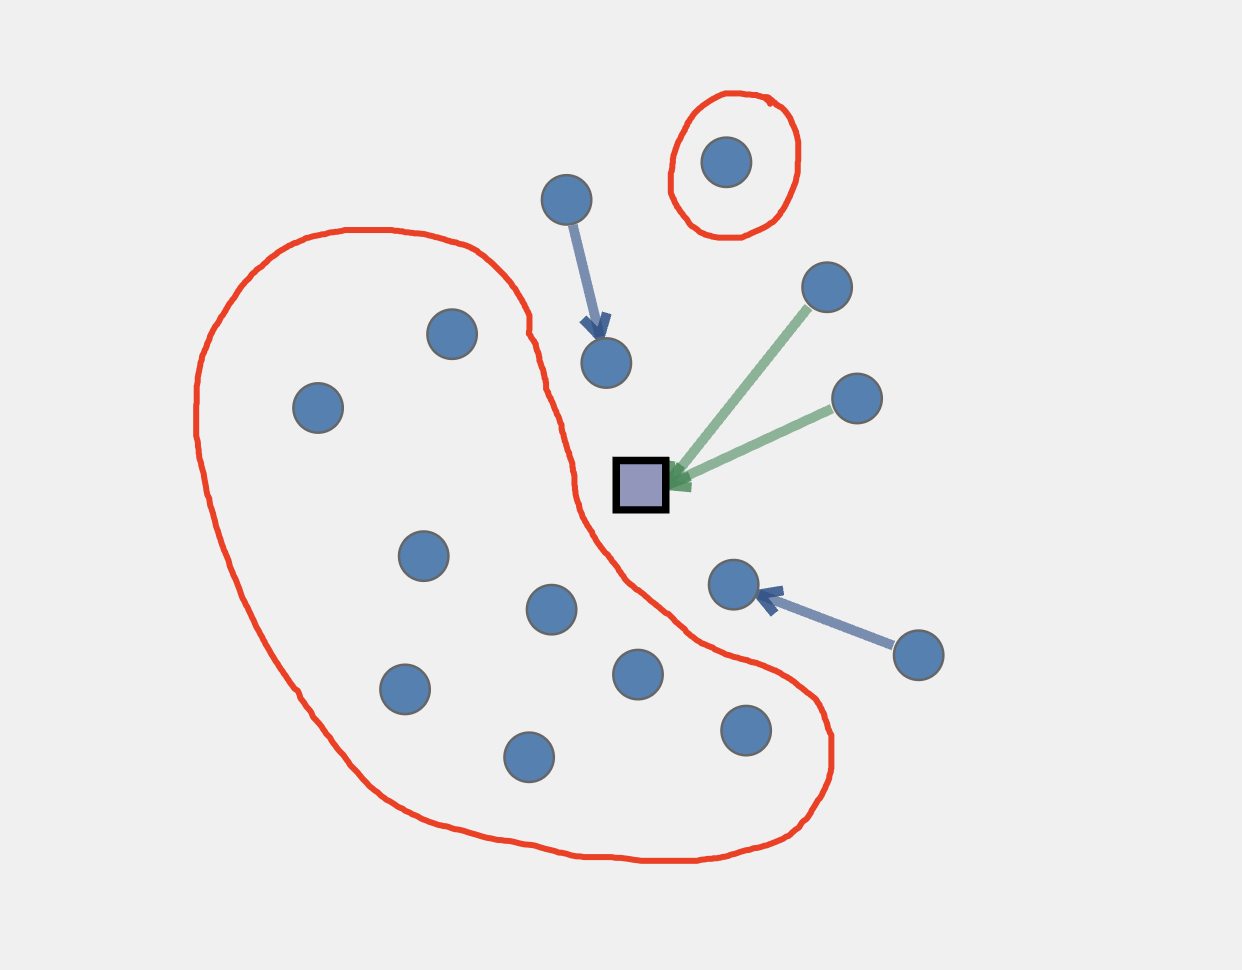
\includegraphics[width=0.4\textwidth]{孤立节点实例.jpg}} % 保留中文标题
    \hspace{2em}
    \subfigure[存在链式调用]{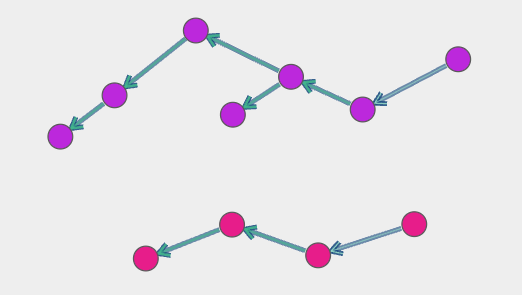
\includegraphics[width=0.4\textwidth]{存在链式调用.jpg}} % 保留中文标题
    \end{minipage}
    \centering
    \begin{minipage}{\textwidth}
    \centering
    \subfigure[antiword-划分模块]{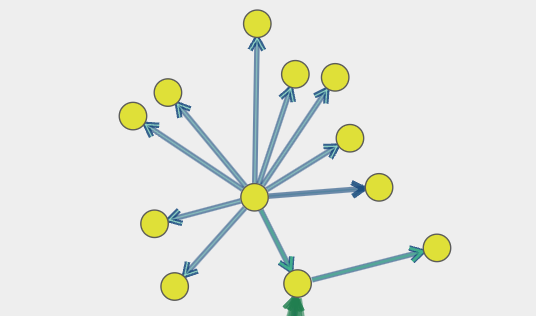
\includegraphics[width=0.4\textwidth]{figures/复杂方法.png}} % 保留中文标题
    \hspace{2em}
    \subfigure[TheAlgorithms-划分模块]{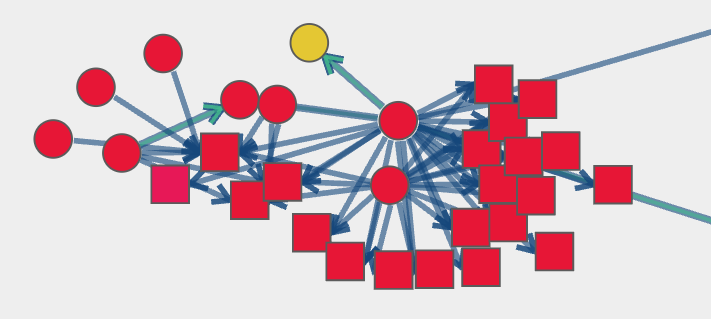
\includegraphics[width=0.4\textwidth]{figures/职责不匹配.png}} % 保留中文标题
    \end{minipage}
    \vspace{0.2em}
    \caption{代码审查图} % 只保留中文标题
\end{figure}



冗余节点

图a表示孤立节点的图模式,图b则是antiword-0.37项目中的实际存在的子图,该图为misc.c 文件的代码审查图。从图中可以清晰地看出,misc.c 文件的结构非常松散,其内部存在大量孤立节点,缺乏足够的联系和协调关系。这种松散的结构正是导致其内聚度表现最差的主要原因。仅依靠代码或文字难以直接反映问题,而配合代码审查图,可以更加直观地展示该模块的结构问题。



长嵌套调用

图a表示嵌套调用的图模式,图b为TheAlgorithms项目中实际存在的子图。



复杂方法

图a表示复杂方法的图模式,图b为antiword-0.37项目中实际存在的子图,我们可以观察到图中的中心节点通过大量出边与其他模块或方法产生关联。



职责不匹配



模块间不良的逻辑型变更影响

图b展示了TheAlgorithms项目中的一个实际子图,涉及两个模块。尽管每个模块的内部结构良好,但各有一个方法与另一模块存在逻辑型影响。这意味着当这些方法发生变动时,不仅当前模块的代码需要修改,其他模块的代码也可能被影响。更为严重的是,随着变更的涟漪效应,这些变更可能扩展并影响更多的代码,导致不必要的连锁反应。

\begin{figure}[!h]
    \setlength{\subfigcapskip}{-1bp}
    \centering
    \begin{minipage}{\textwidth}
    \centering
    \subfigure[模块间不良的逻辑型变更影响图模式]{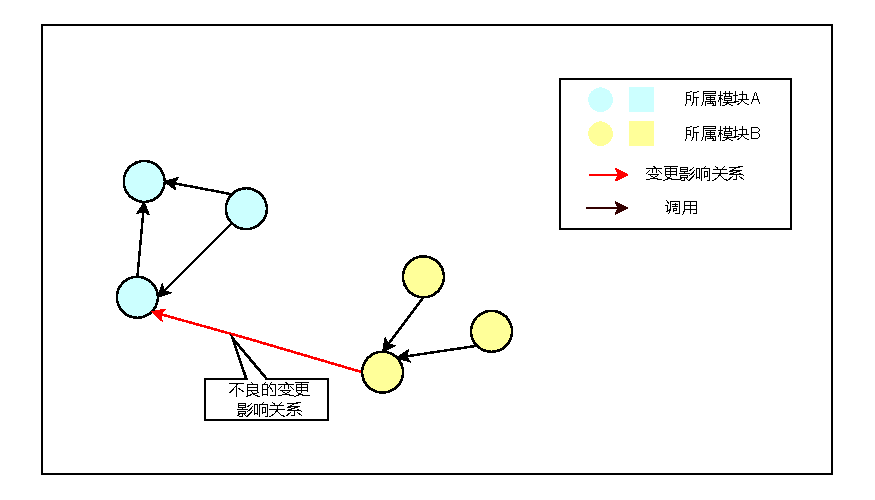
\includegraphics[width=0.45\textwidth]{figures/不良变更影响.pdf}} % 保留中文标题
    \hspace{2em}
    \subfigure[模块间不良的逻辑型变更影响实例]{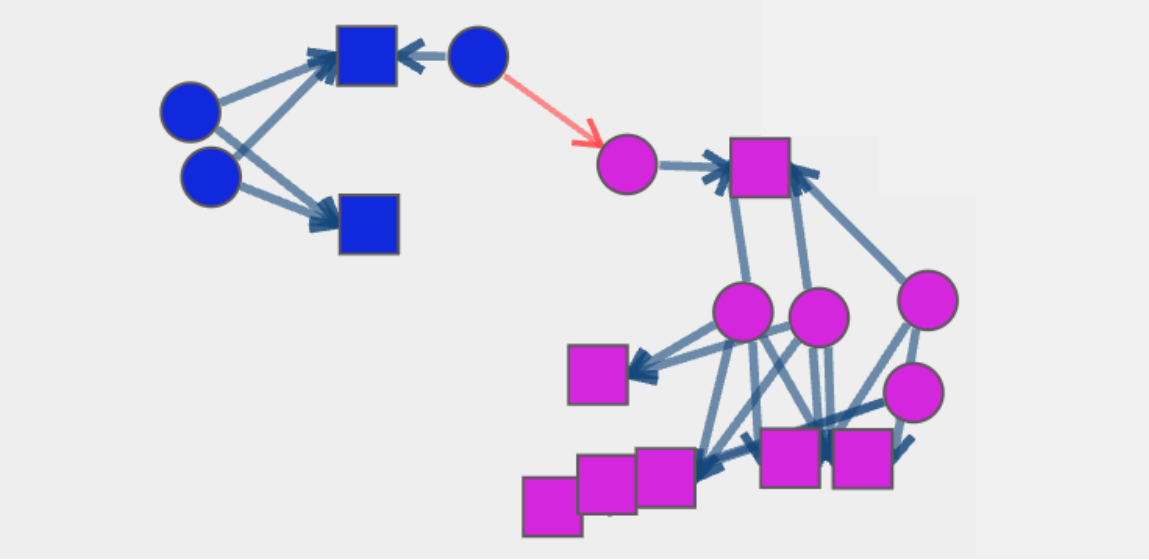
\includegraphics[width=0.45\textwidth]{figures/不良变更影响关系.png}} % 保留中文标题
    \end{minipage}
    \vspace{0.2em}
    \caption{模块间不良的逻辑型变更影响模式及实例} % 只保留中文标题
\end{figure}

总而言之,通过代码审查图,不仅能够帮助开发者快速定位模块质量问题,还能直观地理解问题的根源,为后续的优化和改进提供清晰的建议。这种结合文字与图形的分析方式,显著提升了代码质量评估的直观性和说服力。


\section{代码审查图的应用案例分析}

在实际应用中,代码审查图可以有以下三种用法。

\noindent(1)代码架构可视化能力

图4-8展示了 Antiword 项目和 TheAlgorithms 项目的代码审查图。

\begin{figure}[!h]
    \setlength{\subfigcapskip}{-1bp}
    \centering
    \begin{minipage}{\textwidth}
    \centering
    \subfigure[antiword-未划分模块]{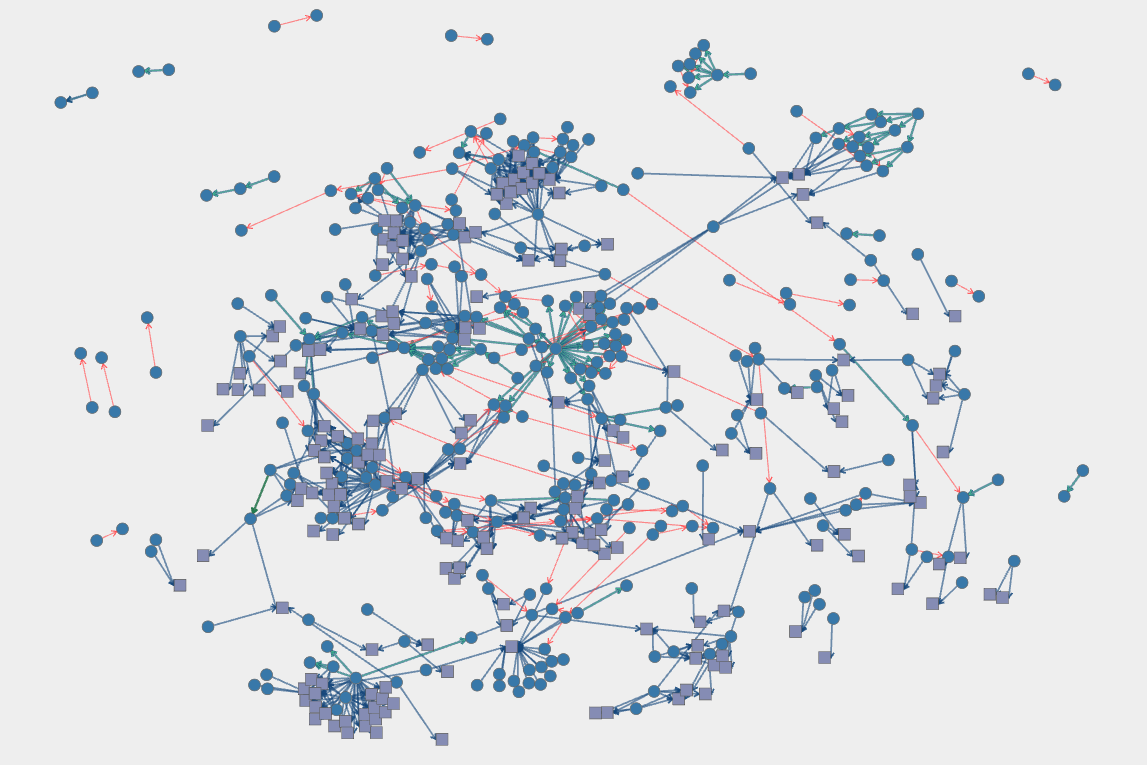
\includegraphics[width=0.4\textwidth]{antiword审查图未上色.jpg}} % 保留中文标题
    \hspace{2em}
    \subfigure[TheAlgorithms-未划分模块]{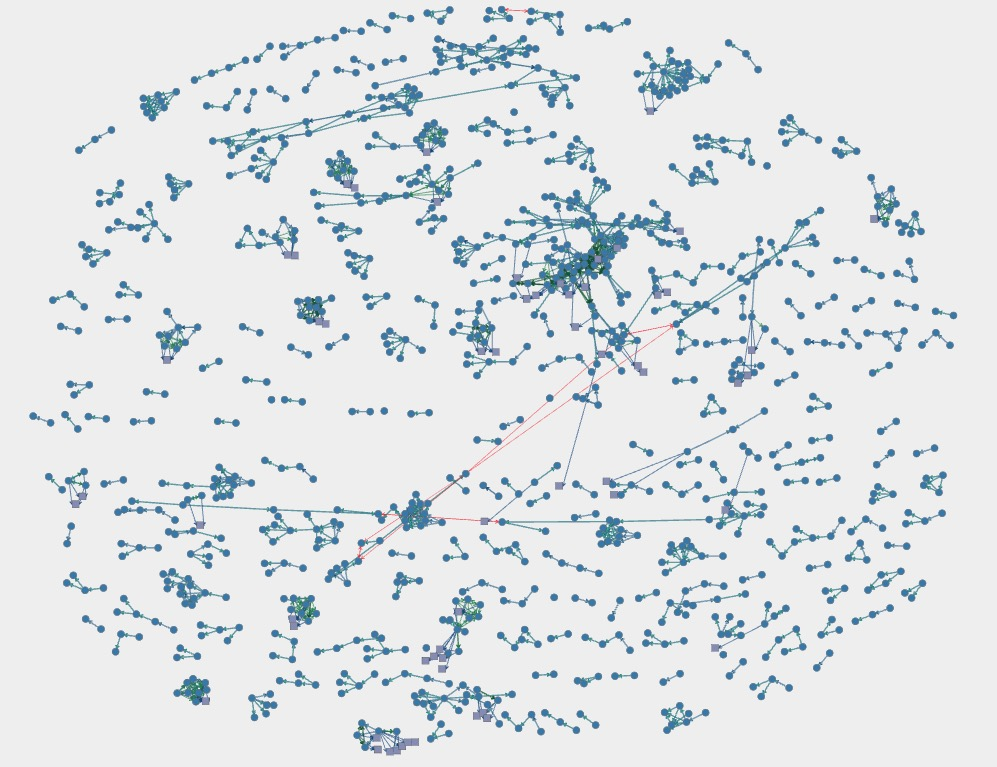
\includegraphics[width=0.4\textwidth]{aigri代码审查图-未上色.jpg}} % 保留中文标题
    \end{minipage}
    \centering
    \begin{minipage}{\textwidth}
    \centering
    \subfigure[antiword-划分模块]{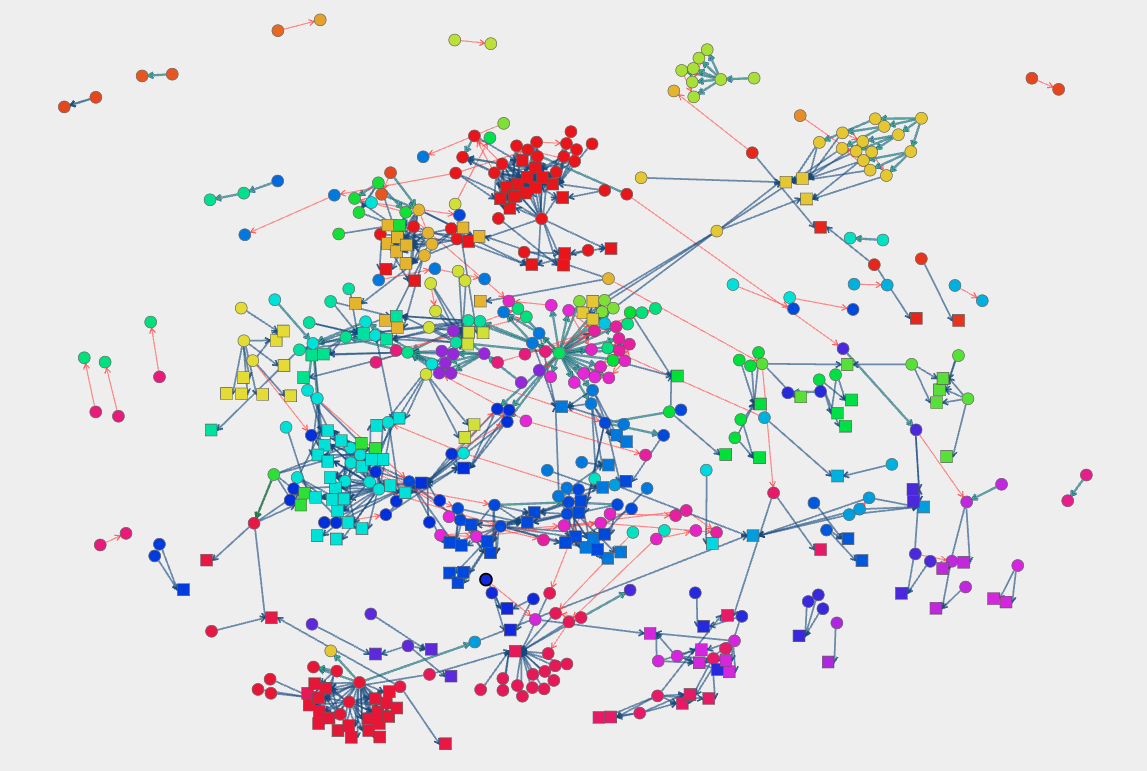
\includegraphics[width=0.4\textwidth]{antiword代码审查图.jpg}} % 保留中文标题
    \hspace{2em}
    \subfigure[TheAlgorithms-划分模块]{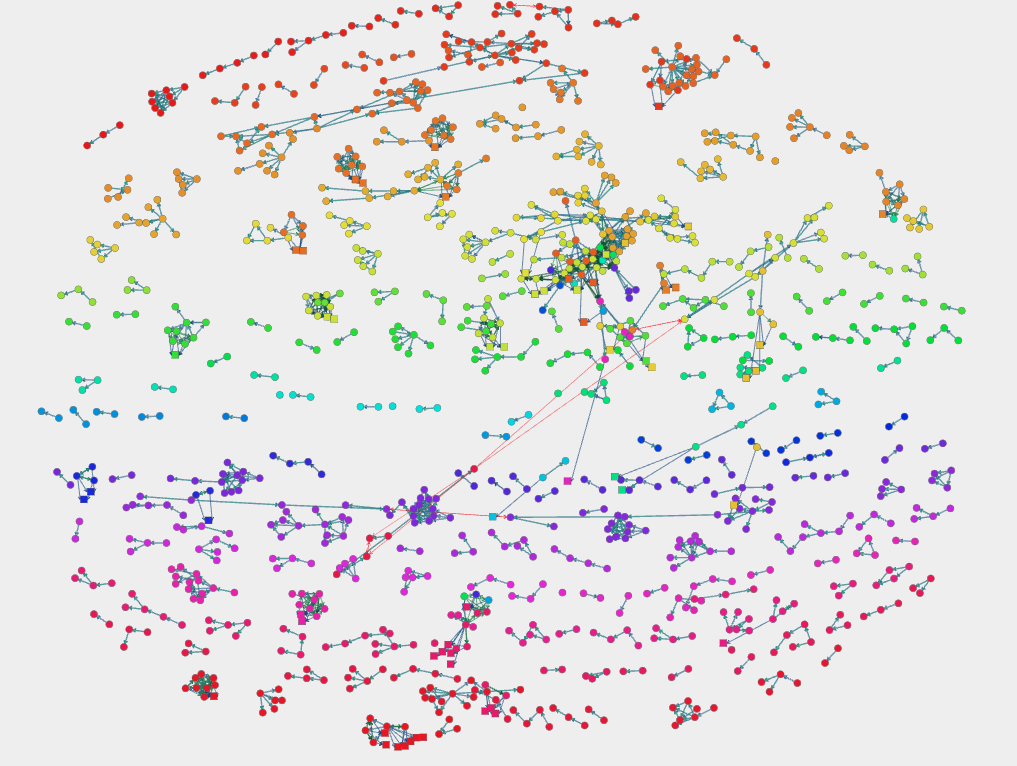
\includegraphics[width=0.4\textwidth]{aigri代码审查图.jpg}} % 保留中文标题
    \end{minipage}
    \vspace{0.2em}
    \caption{代码审查图} % 只保留中文标题
\end{figure}


图中圆形节点表示方法,方形节点表示全局变量,不同颜色的边则代表了代码元素之间的不同关系:蓝色边表示依赖关系,绿色边表示耦合关系,红色边表示代码变更影响关系。图a和图b是未区分模块的全局视图,图c和图d则对模块进行了区分,采用颜色区分不同模块,将属于同一模块的节点用相同颜色进行标注,从而进一步突出模块之间的边界和逻辑关系。

\paragraph{结构特征信息} 从图中可以明显看出两个项目在结构特征上的显著差异。
\begin{itemize}
    \item Antiword 项目整体模块之间高度协作,共同实现一个完整的功能,因此模块之间的联系较为紧密,表现出较强的耦合性。从可视化图上观察,按模块划分后,可以清晰地看到具有相同功能的模块形成了较为紧密的聚集。同一颜色的节点集中分布,进一步体现了模块的内聚性较高以及逻辑结构的清晰性。
    
    \item TheAlgorithms 项目由于其作为算法库的特性,方法之间的耦合性较低,各模块间的联系相对较弱。从图上来看,不同模块呈现出较为分散的分布,模块内部的聚集程度也较低。整体结构表现为由若干独立模块组成,松散而分离,符合库函数式项目的典型特征。
\end{itemize}

\paragraph{代码度量信息} 点击图中的某个节点可查看该节点的详细信息,包括方法或全局变量的具体描述,以及代码度量信息。这一功能能够帮助用户快速了解特定方法或变量的功能和用途,并根据代码度量信息了解方法或所在模块的质量情况,从而更高效地进行代码审查和理解。


\begin{figure}[h]
\centering
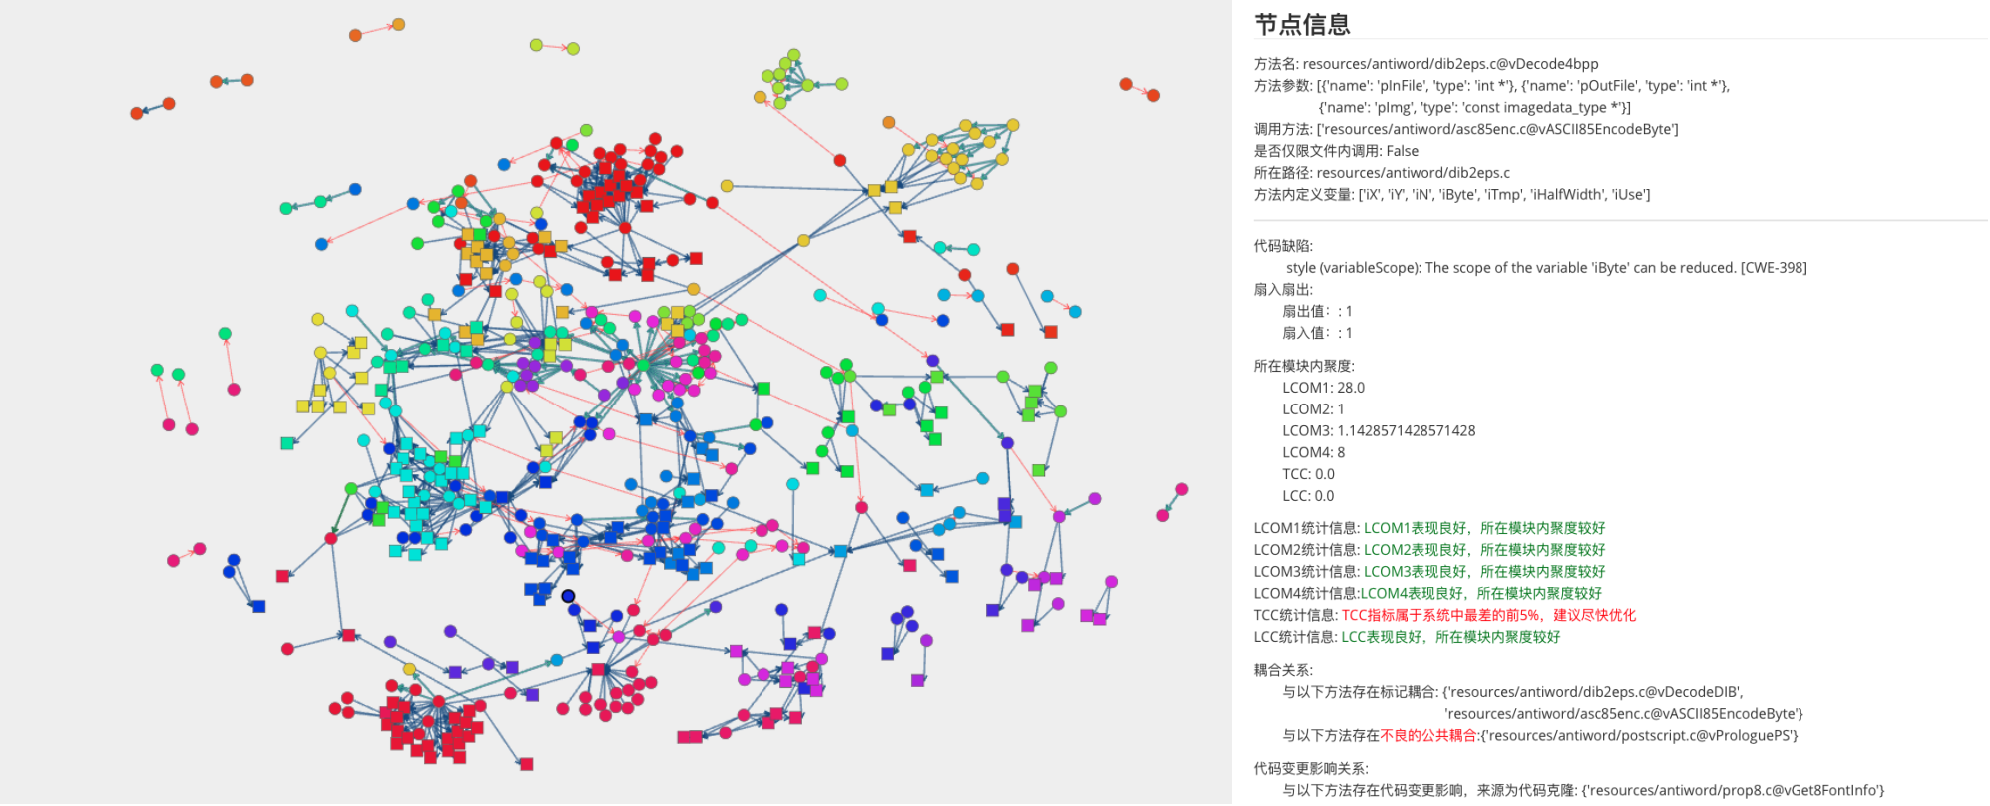
\includegraphics[width = 1\textwidth]{点击节点.png}
\caption{点击节点展开节点信息}
\end{figure}


\noindent(2)图构助读能力

代码审查图蕴含了很多丰富有价值的信息,通过聚焦于代码审查图中的子图,用户可以快速直观地理解其所关注的代码结构之间的关系。子图清晰地展示了代码结构之间的依赖、耦合以及变更影响关系,使得复杂的代码逻辑更加直观。

这里聚焦于 antiword 项目中的vDecodeDIB 方法的代码开发和审查场景。若按照传统方法对该方法进行开发或分析,人工阅读代码需要涉及 300 多行代码的逻辑才能全面掌握方法的上下文。然而,通过代码审查图,开发者只需关注 8 个节点和 9 条边,即可快速获取关键信息。这种直观的可视化显著降低了代码理解的复杂度和成本。

\begin{figure}[h]
\centering
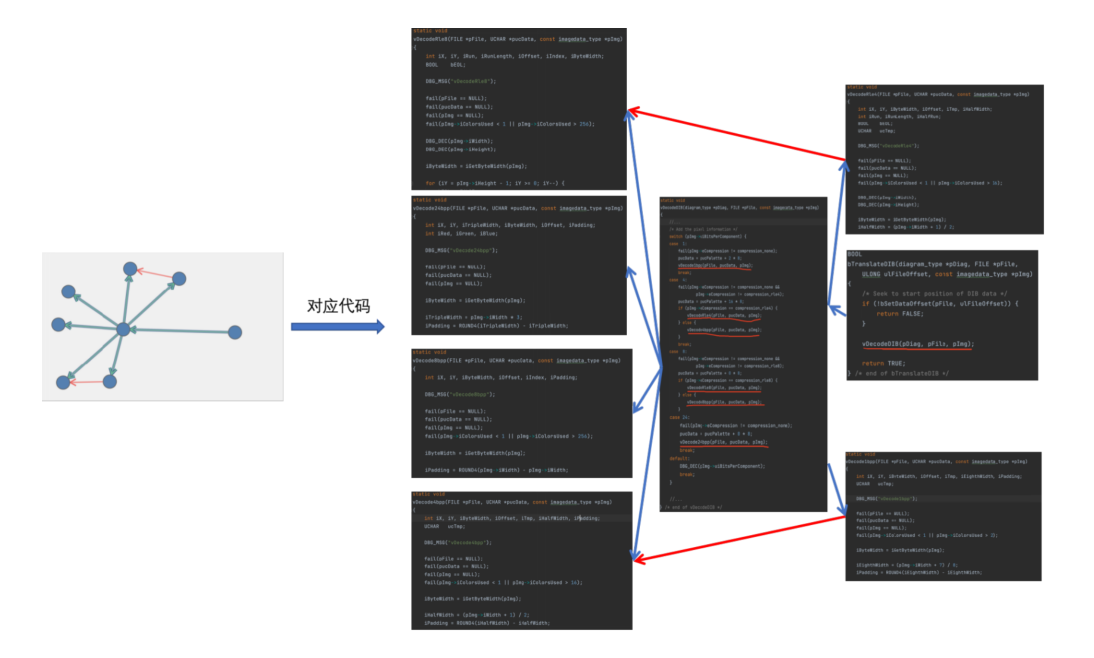
\includegraphics[width = 1\textwidth]{代码审查图子图.jpg}
\caption{vDecodeDIB方法上下文}
\end{figure}

尤其值得注意的是,该方法的上下文中包含了两个基于克隆代码的变更影响关系。这类关系通常隐匿于代码中,开发者仅靠手动查看代码很难准确发现并更改。代码审查图将这些隐藏的逻辑变更影响关系显式标出,使开发者在代码修改时能够快速识别潜在的影响范围,从而避免遗漏变更的风险。

\paragraph{辅助开发者的代码维护} 当用户对软件代码进行开发时,可将复杂庞大的项目先通过系统进行分析,得到代码审查图。

\begin{figure}[h]
\centering
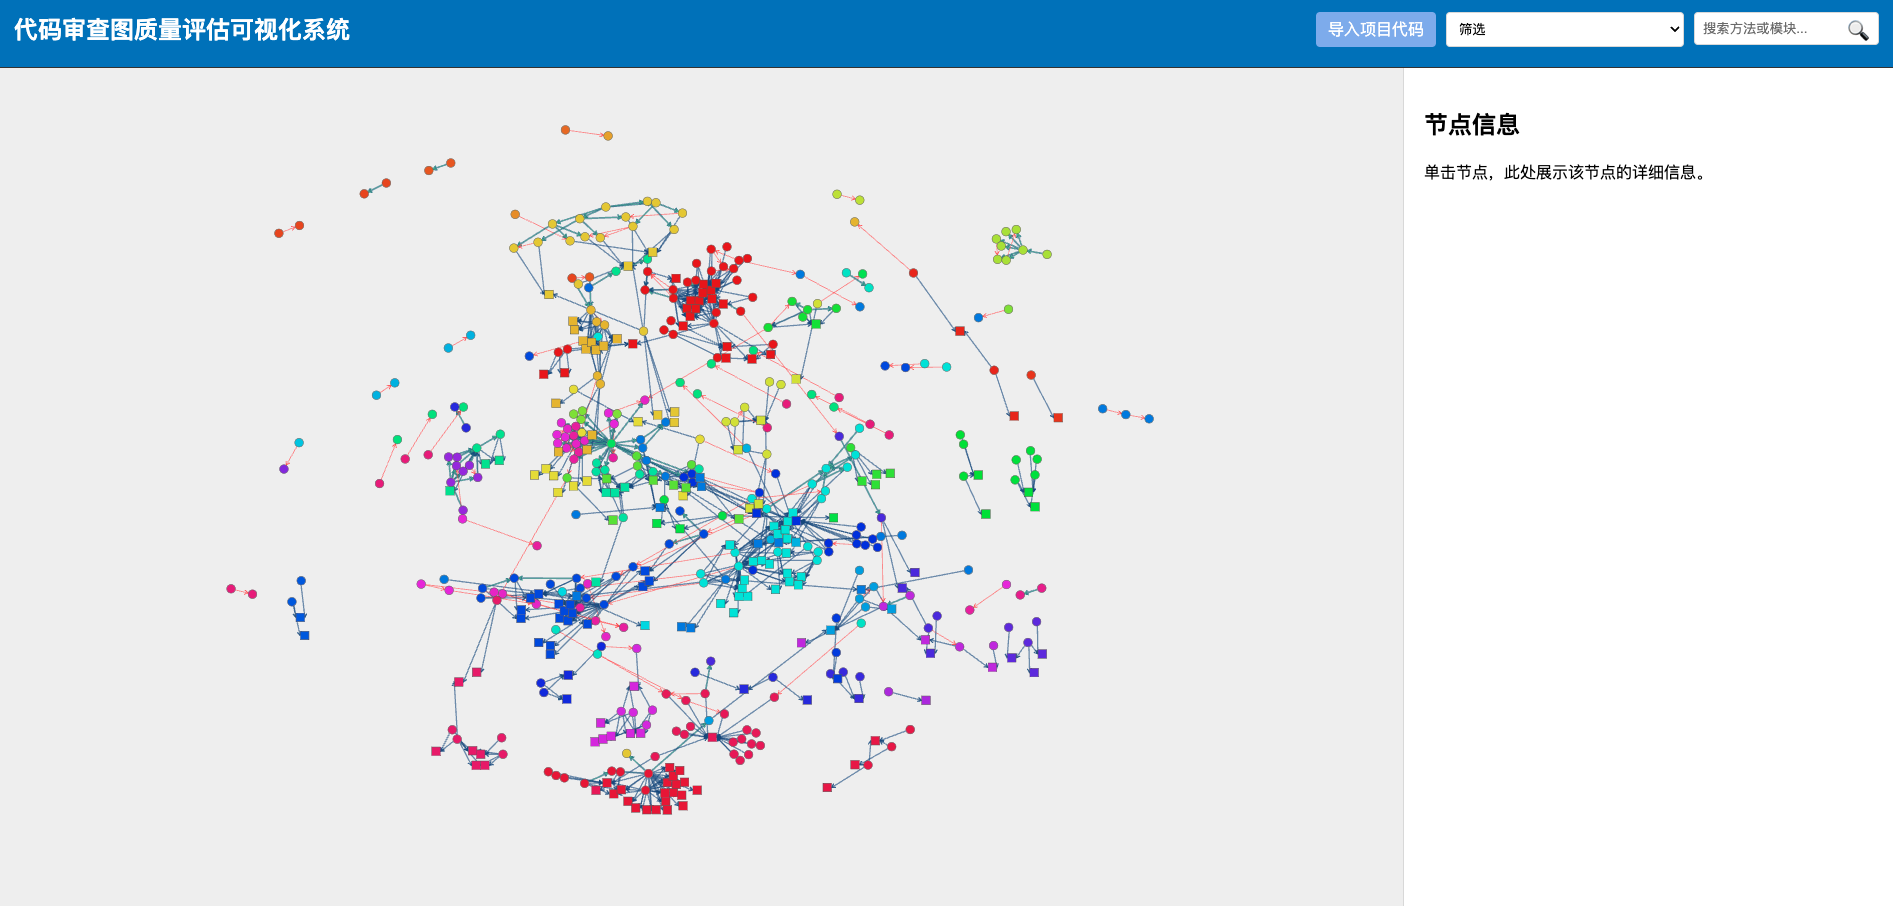
\includegraphics[width = 1.0\textwidth]{应用展示审查图.jpg}
\caption{导入项目生成代码审查图}
\end{figure}

对于开发任务所在的代码上下文,通过搜索方法名找到其在代码审查图中的位置,点击节点查看方法详细信息和质量情况,用户可根据相应的建议进行修改,优化代码质量。

\begin{figure}[h]
\centering
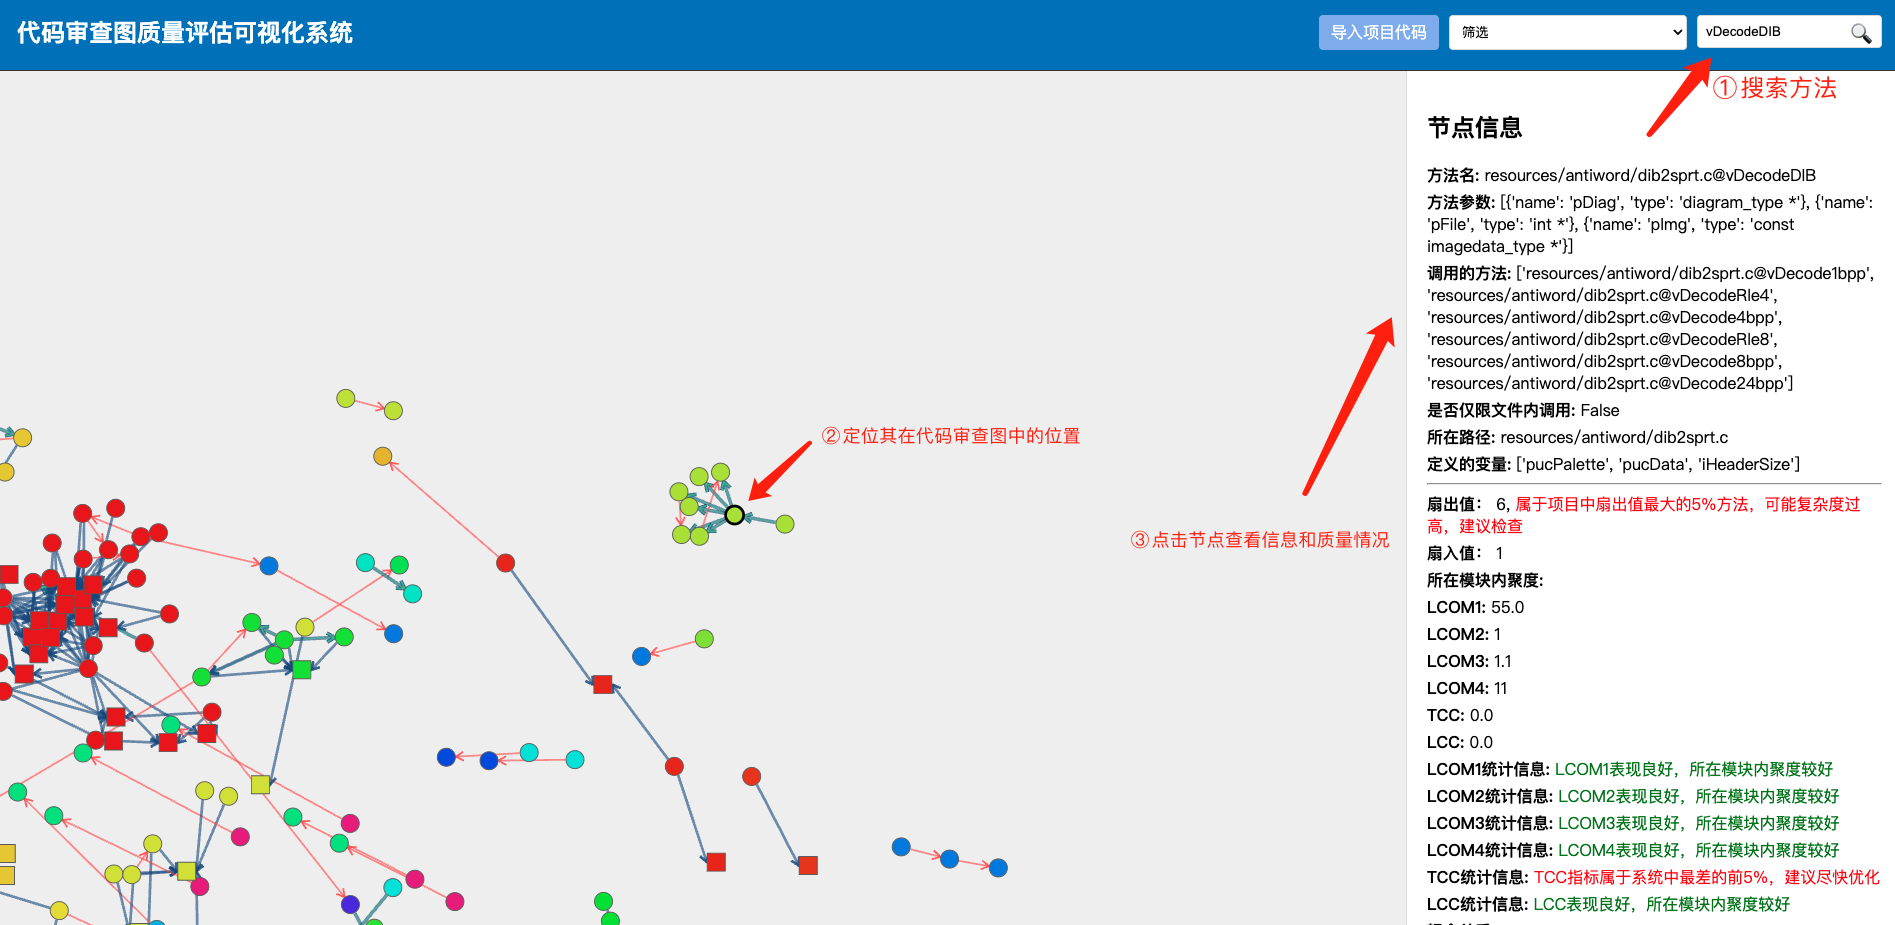
\includegraphics[width = 1.0\textwidth]{应用查看节点信息.jpg}
\caption{定位开发任务涉及的方法,查看质量信息}
\end{figure}

根据代码审查图的边,则可以了解当前代码与其他部分的依赖关系、耦合关系和变更影响关系。尤其是变更影响关系,可以帮助用户在进行变更时,提示其依赖型和逻辑型影响的范围,并根据给出的建议,帮助用户安全变更,解决了用户面对复杂软件难以理解、不敢变更、容易变更不完全的痛点。

\begin{figure}[h]
\centering
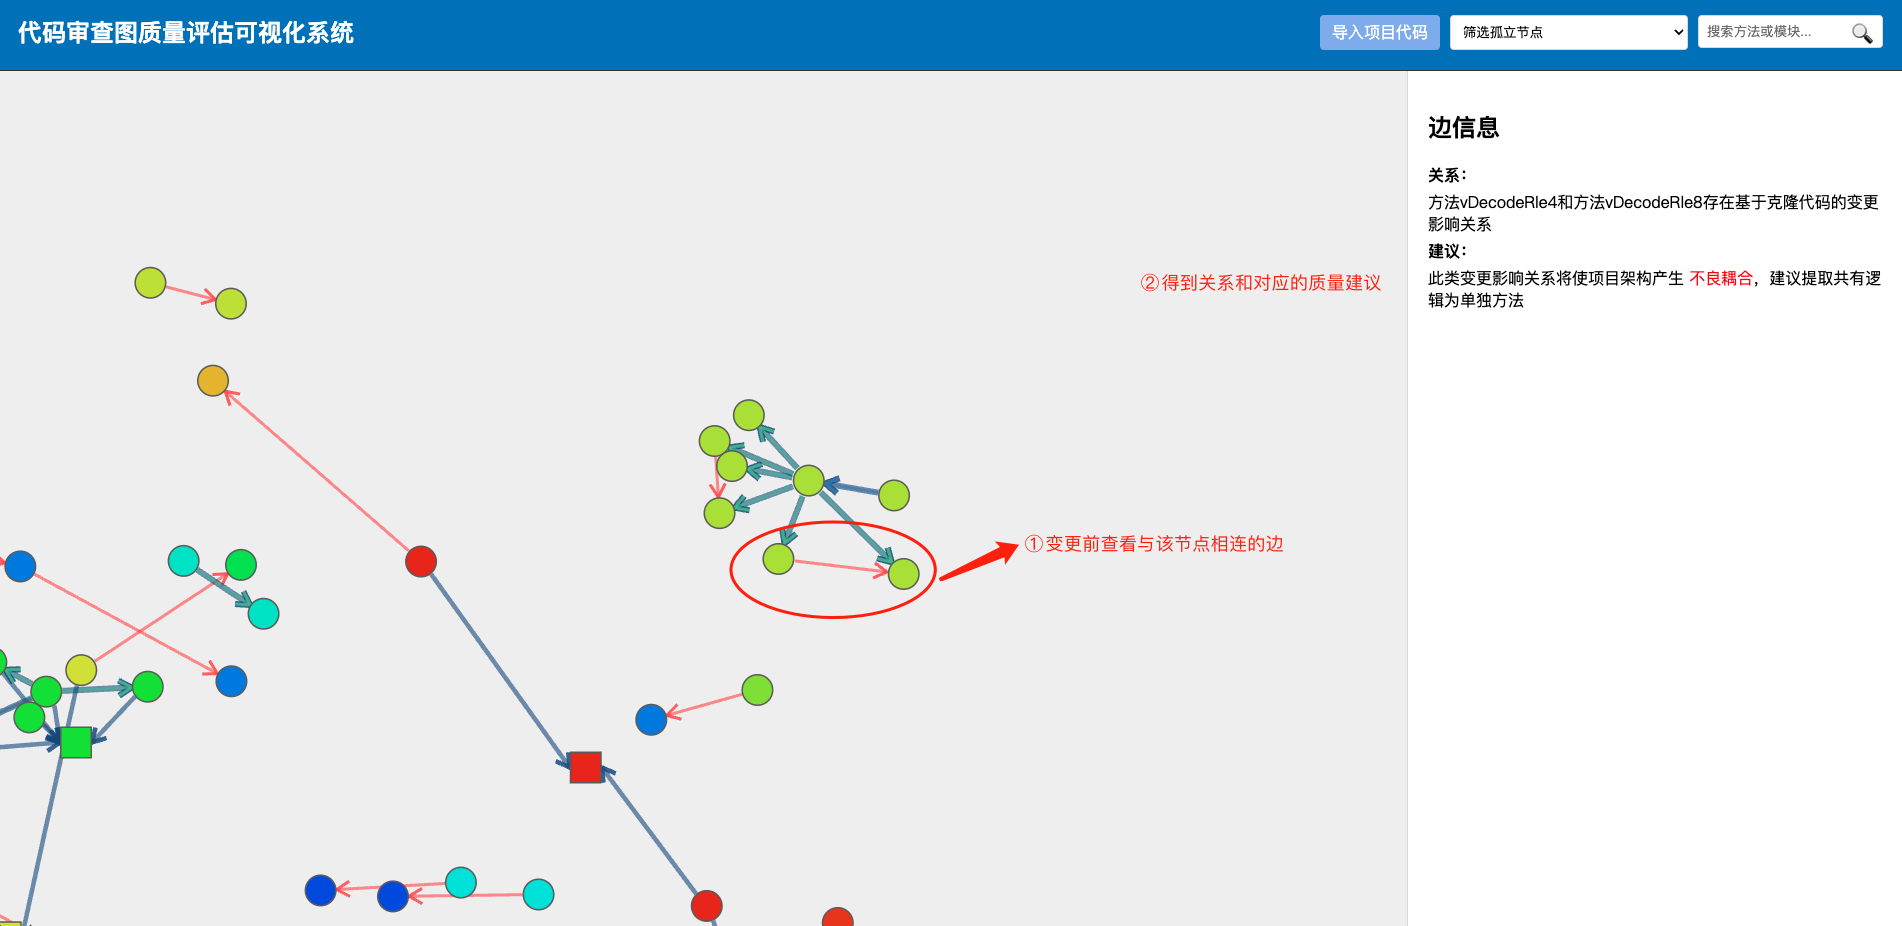
\includegraphics[width = 1.0\textwidth]{应用边信息.jpg}
\caption{查看方法对应边,按建议安全变更}
\end{figure}

\paragraph{作为审查工具帮助审查者进行审查} 当面对审查任务时,审查者可通过搜索代码审查图定位到当前提交所涉及的节点,通过图中的关系迅速了解代码上下文间的调用以及变更影响关系,通过系统的提示,对开发者的变更进行审查,检查其功能逻辑上是否安全变更,检查其变更操作给软件带来的质量影响是恶化还是优化,从而给出对应的审查结果。

\paragraph{作为质量评估工具对软件代码进行整体的评估} 用户可根据代码审查图,观察软件模块划分,也可导出代码质量评估报告,以清单的方式了解项目代码的质量情况。



\section{本章小结}

本章首先提出了一个代码质量度量模型,并结合可视化的代码审查图对软件架构和代码质量度量进行了宏观展示。通过这种可视化方式,用户能够更直观地了解代码的质量状况,并通过导出代码质量分析报告来方便地进行查询和进一步分析。最后,实验结果验证了该代码质量度量模型能够有效地反映代码的相对质量水平,证明了代码审查图在实际应用中的价值。此外还总结了五种常见的不良图模式,帮助用户更好地理解代码质量问题,并为代码重构提供了有效的参考依据。
